% JULIE 
\begin{frame}
\frametitle{Betydning af parametrene}
\begin{itemize}
\item Fordobling af $\alpha$
\end{itemize}

\begin{minipage}{0.49\textwidth}
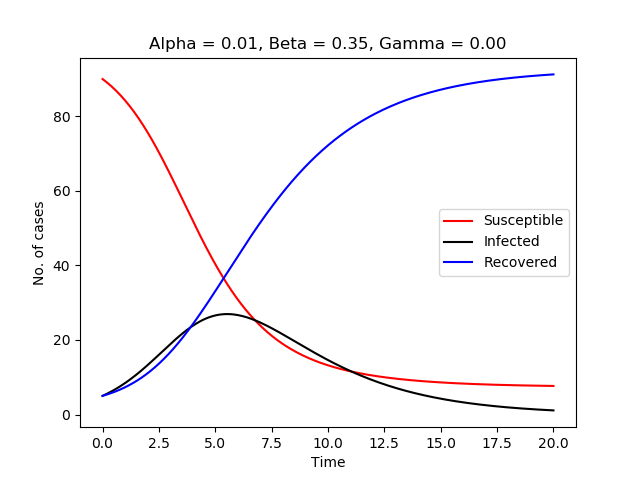
\includegraphics[scale=0.3]{fig/img/t_a1_b35_g0.png}
\end{minipage}
%
\begin{minipage}{0.49\textwidth}
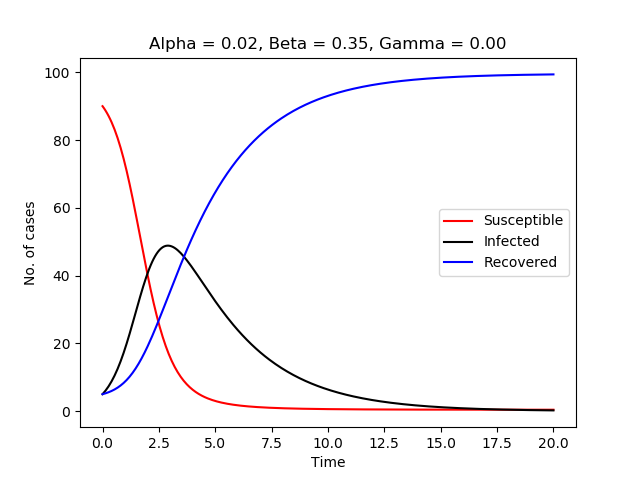
\includegraphics[scale=0.3]{fig/img/t_a2_b35_g0.png}
\end{minipage}
\end{frame}
%
\begin{frame}
\frametitle{Betydning af parametrene}
\begin{itemize}
\item Fordobling af $\beta$
\end{itemize}

\begin{minipage}{0.49\textwidth}
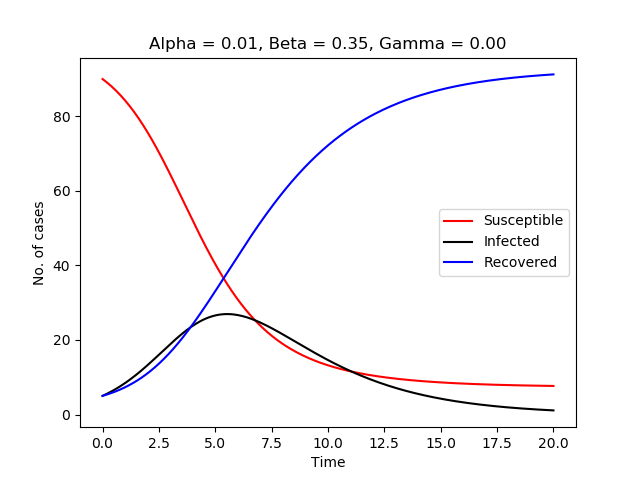
\includegraphics[scale=0.3]{fig/img/t_a1_b35_g0.png}
\end{minipage}
%
\begin{minipage}{0.49\textwidth}
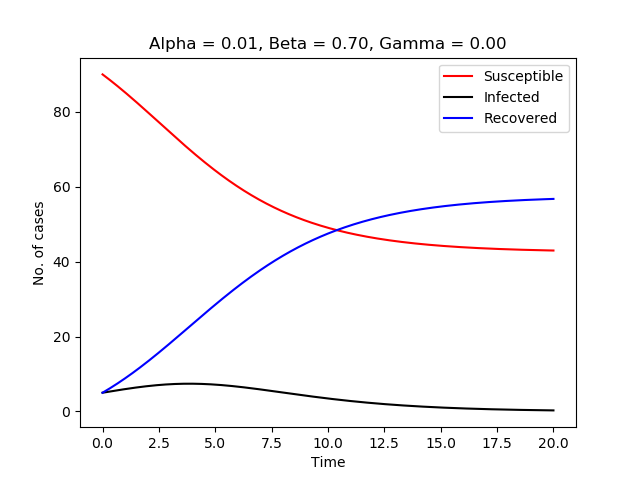
\includegraphics[scale=0.3]{fig/img/t_a1_b7_g0.png}
\end{minipage}
\end{frame}
%
% MADS 
\begin{frame}
\frametitle{Betydning af parametrene}
\begin{itemize}
\item $x_{1,0}$ fra 90 til 85
\item Fordobling af antal immune
\end{itemize}

\begin{minipage}{0.49\textwidth}
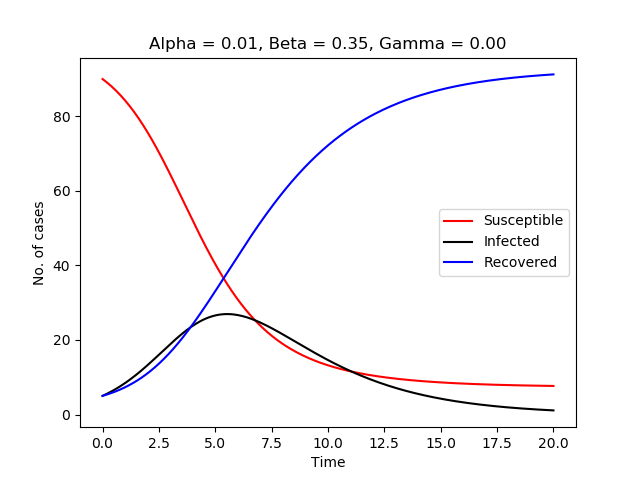
\includegraphics[scale=0.3]{fig/img/t_a1_b35_g0.png}
\end{minipage}
%
\begin{minipage}{0.49\textwidth}
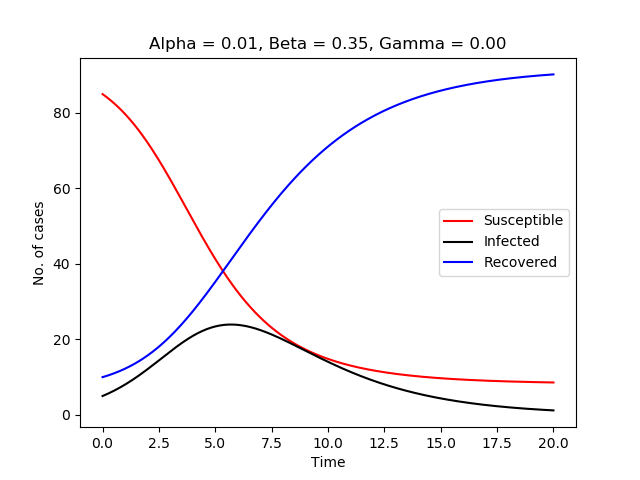
\includegraphics[scale=0.3]{fig/img/t_x1_5_x2_85.png}
\end{minipage}
\end{frame}
%
\begin{frame}
\frametitle{Betydning af parametrene}
\begin{itemize}
\item Ændring af indledende syge, $x_{2,0}$, fra $5$ til $1$
\end{itemize}

\begin{minipage}{0.49\textwidth}
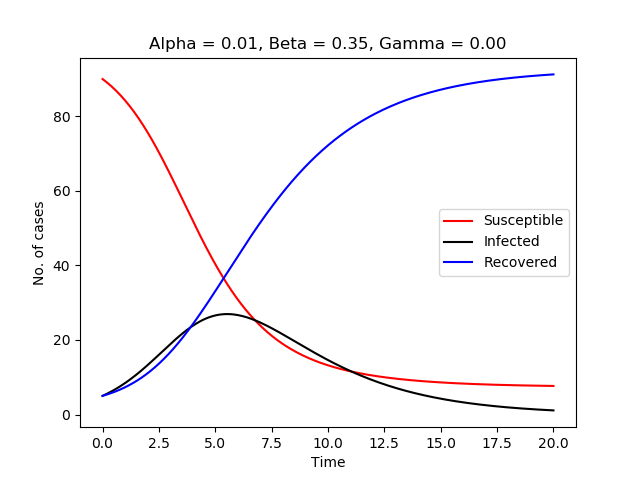
\includegraphics[scale=0.3]{fig/img/t_a1_b35_g0.png}
\end{minipage}
%
\begin{minipage}{0.49\textwidth}
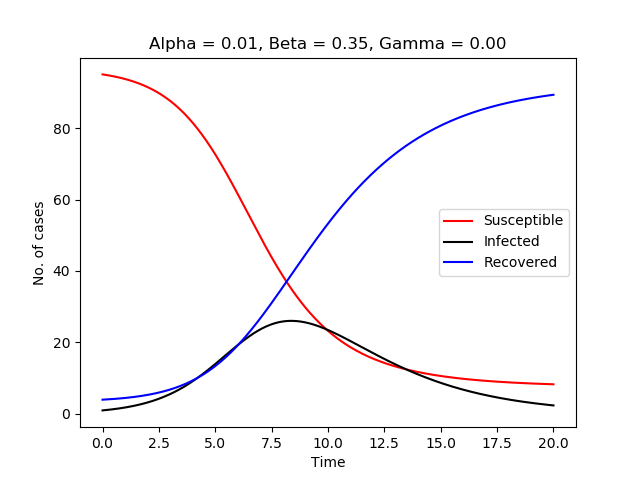
\includegraphics[scale=0.3]{fig/img/t_x1_1_x2_95.png}
\end{minipage}
\end{frame}
%

